% 原章第44页6.3至第50页6.4标题前，式6.152—6.167。
\section{用于影像数据降维的二维或三维函数主成分分析}

影像信号的降维，在图像分类和影像遗传学分析中都很重要（Su et al. 2017）。常用降维方法包括主成分分析（PCA）、决策边界特征提取（decision boundary feature extraction，DBFE）、非负矩阵分解与判别分析特征提取（discriminative analysis feature extraction，DAFE）（Diwaker and Dutta 2015）。然而，这些方法未利用图像内部的空间信息。为克服这些局限、充分利用空间信息与谱信息，将一维函数主成分分析（functional principal component analysis，FPCA）推广为二维 FPCA（Lin et al. 2015）。本节主要介绍三维 FPCA，二维 FPCA 可视为其特例。

\subsection{问题表述}

与 PCA 类似，考虑函数值的线性组合：
\begin{equation}
f=\int_S\int_T\int_U\beta(s,t,u)x(s,t,u)\,ds\,dt\,du,
\tag{6.152}
\end{equation}
其中，$\beta(s,t,u)$ 为权函数，$x(s,t,u)$ 为中心化随机函数，例如图像的强度函数。为捕捉随机函数中的变异，选择使 $f$ 的方差最大的权函数 $\beta(s,t,u)$。根据随机积分的方差公式（Henderson and Plaschko 2006），有
\begin{equation}
\begin{aligned}
\operatorname{var}(f)&=\int_S\int_T\int_U\int_S\int_T\int_U,\ \beta(s_1,t_1,u_1)R(s_1,t_1,u_1,s_2,t_2,u_2)\\
&\qquad\beta(s_2,t_2,u_2)\,ds_1\,dt_1\,du_1\,ds_2\,t_2\,du_2,
\end{aligned}\tag{6.153}
\end{equation}
其中，$R(s_1,t_1,u_1,s_2,t_2,u_2)=\operatorname{cov}(x(s_1,t_1,u_1),x(s_2,t_2,u_2))$ 为 $x(s,t,u)$ 的协方差函数。定义扩展内积为
\[
\begin{aligned}
(f,g)_\mu&=\int_S\int_T\int_U f(s,t,u)g(s,t,u)\,ds\,dt\,du\\
&\quad+\mu\int_S\int_T\int_U\frac{\partial^6 f(s,t,u)}{\partial s^2\,\partial t^2\,\partial u^2}
\frac{\partial^6 g(s,t,u)}{\partial s^2\,\partial t^2\,\partial u^2}\,ds\,dt\,du.
\end{aligned}
\]
由于将 $\beta(s,t,u)$ 乘以常数不会改变方差 $\operatorname{Var}(f)$ 的极大化解，施加以下约束，使解唯一：
\begin{equation}
\int_S\int_T\int_U\beta^2(s,t,u)\,ds\,dt+\mu\int_S\int_T\int_U
\left[\frac{\partial^6\beta(s,t,u)}{\partial s^2\,\partial t^2\,\partial u^2}\right]^2\,ds\,dt\,du=1.
\tag{6.154}
\end{equation}
因此，为求权函数，需解以下优化问题：
\begin{equation}
\begin{aligned}
\operatorname{Max}\quad&\int_S\int_T\int_U\int_S\int_T\int_U\beta(s_1,t_1,u_1)R(s_1,t_1,u_1,s_2,t_2,u_2)\\
&\qquad\beta(s_2,t_2,u_2)\,ds_1\,dt_1\,du_1\,ds_2\,t_2\,du_2\\
\text{s.t.}\quad&\int_S\int_T\int_U\beta^2(s,t,u)\,ds\,dt\\
&\quad+\mu\int_S\int_T\int_U\left[\frac{\partial^6\beta(s,t,u)}{\partial s^2\,\partial t^2\,\partial u^2}\right]^2\,ds\,dt\,du=1.
\end{aligned}\tag{6.155}
\end{equation}

\subsection{积分方程与特征函数}

利用拉格朗日乘子，将约束优化问题 (6.155) 改写为以下无约束优化问题：
\begin{equation}
\begin{aligned}
\max_\beta\quad&\frac12\int_S\int_T\int_U\int_S\int_T\int_U\beta(s_1,t_1,u_1)R(s_1,t_1,u_1,s_2,t_2,u_2)\\
&\qquad\beta(s_2.\ t_2,u_2)\,ds_1\,dt_1\,ds_2\,t_2\\
&+\frac12\lambda\Biggl(1-\int_S\int_T\int_U\beta^2(s_1,t_1,u_1)\,ds_1\,dt_1\,du_1\\
&\qquad-\mu\int_S\int_T\int_U\left[\frac{\partial^6\beta(s_1,t_1,u_1)}{\partial s_1^2\,\partial t_1^2\,\partial u_1^2}\right]^2\,ds_1\,dt_1\,du_1\Biggr),
\end{aligned}\tag{6.156}
\end{equation}
其中，$\lambda$ 为参数。根据变分法（Sagan 2012），定义泛函
\[
\begin{aligned}
J[\beta]&=\frac12\int_S\int_T\int_U\int_S\int_T\int_U\beta(s_1,t_1,u_1)R(s_1,t_1,u_1,s_2,t_2,u_2)\\
&\qquad\beta(s_2.\ t_2)\,ds_1\,dt_1\,ds_2\,t_2\\
&\quad+\frac12\lambda\left(1-\int_S\int_T\int_U\beta^2(s_1,t_1,u_1)\,ds_1\,dt_1\,du_1\right)\\
&\quad-\mu\int_S\int_T\int_U\left[\frac{\partial^6\beta(s_1,t_1,u_1)}{\partial s_1^2\,\partial t_1^2\,\partial u_1^2}\right]^2\,ds_1\,dt_1\,du_1).
\end{aligned}
\]
其一阶变分为
\[
\begin{aligned}
\delta J[h]&=\frac d{d\varepsilon}J[\beta(s,t,u)+\varepsilon h(s,t,u)]\\
&=\int_S\int_T\int_U\Biggl[\int_S\int_T\int_U\Biggl[R(s_1,t_1,u_1,s_2,t_2,u_2)\beta(s_2,t_2,u_2)\,ds_2\,t_2\,du_2\\
&\qquad-\lambda\left(\beta(s_1,t_1,u_1)+\mu\frac{\partial^{12}\beta(s_1,t_1,u_1)}{\partial s_1^4\,\partial t_1^4\,\partial u_1^4}\right)\Biggr]h(s_1,t_1,u_1)\,ds_1\,dt_1\,du_1\\
&=\int_S\int_T\int_U\Biggl[\int_S\int_T\int_U R(s_1,t_1,u_1,s_2,t_2,u_2)\beta(s_2,t_2,u_2)\,ds_2\,dt_2\,du_2\\
&\qquad-\lambda\left(\beta\biggl(s_1,t_1,u_1+\mu\frac{\partial^{12}\beta(s_1,t_1,u_1)}{\partial s_1^4\,\partial t_1^4\,\partial u_1^4}\biggr)\right)\Biggr]^2\,ds_1\,dt_1\,du_1=0,
\end{aligned}
\]
由此得到以下积分方程：
\begin{equation}
\begin{aligned}
&\int_S\int_T\int_U R(s_1,t_1,u_1,s_2,t_2,u_2)\beta(s_2,t_2,u_2)\,ds_2\,dt_2\,du_2\\
&\qquad=\lambda\left[\beta(s_1,t_1,u_1)+\mu\frac{\partial^{12}\beta(s_1,t_1,u_1)}{\partial s_1^4\,\partial t_1^4\,\partial u_1^4}\right],
\end{aligned}\tag{6.157}
\end{equation}
其中，$\lambda$ 为适当的特征值。积分方程 (6.157) 左端定义了权函数 $\beta$ 的三维积分变换 $R$。因此，协方差函数 $R(s_1,t_1,u_1,s_2,t_2,u_2)$ 的积分变换称为协方差算子 $R$。积分方程 (6.157) 可改写为
\begin{equation}
R\beta=\lambda\beta,
\tag{6.158}
\end{equation}
其中，$\beta(s_1,t_1,u_1,s_2,t_2,u_2)$ 为特征函数，称为主成分函数。式 (6.158) 也称为三维特征方程。显然，若将协方差算子与特征函数分别替换为协方差矩阵与特征向量，则式 (6.158) 的形式与多元 PCA 的特征方程相同。

理论上函数值的数目为无穷，因此可能有无穷多个特征值。只要函数 $X_i$ 与 $Y_i$ 不线性相关，就只有 $N-1$ 个非零特征值，其中 $N$ 为抽样个体总数（$N=n_A+n_G$）。满足特征方程的特征函数正交归一（Ramsay and Silverman 2005）。换言之，式 (6.158) 生成一组主成分函数
\[
R\beta_k=\lambda_k\beta_k,\qquad\lambda_1\geq\lambda_2\geq\cdots.
\]
这些主成分函数满足：
\begin{enumerate}[label=\arabic*.]
\item
\[
\int_S\int_T\int_U\beta_k^2(s,t,u)\,ds\,dt\,du+\mu\int_S\int_T\int_U
\left[\frac{\partial^6\beta_k(s,t,u)}{\partial s^2\,\partial t^2\,\partial u^2}\right]^2\,ds\,dt\,du=1.
\]
\item 对所有 $m<k$，
\[
\begin{aligned}
&\int_S\int_T\int_U\beta_k(s,t,u)\beta_m(s,t,u)\,ds\,dt\,du\\
&\quad+\mu\int_S\int_T\int_U\frac{\partial^6\beta_k(s,t,u)}{\partial s^2\,\partial t^2\,\partial u^2}
\frac{\partial^6\beta_m(s,t,u)}{\partial s^2\,\partial t^2\,\partial u^2}\,ds\,dt\,du=0.
\end{aligned}
\]
\end{enumerate}
最大特征值对应的主成分函数 $\beta_1$ 称为第一主成分函数，第二大特征值对应的主成分函数 $\beta_2$ 称为第二主成分函数。

\subsection{函数主成分函数与函数主成分得分的计算}

特征函数是一个积分函数，难以得到闭式解。求解特征函数问题的一般策略，是将连续特征分析问题转化为适当的离散特征分析任务（Ramsay and Silverman 2005）。这里使用基函数展开方法实现这种转换。

令 $\{\phi_j(t)\}$ 为傅里叶函数系。对各个 $j$，定义 $\omega_{2j-1}=\omega_{2j}=2\pi j$。将每个函数 $x_i(s,t,u)$ 展开为基函数 $\phi_j$ 的线性组合：
\begin{equation}
x_i(s,t,u)=\sum_{j=1}^K\sum_{k=1}^K\sum_{l=1}^Kc_{jkl}^{(i)}\phi_j(s)\phi_k(t)\phi_l(u).
\tag{6.159}
\end{equation}
令
\[
tC_i=[c_{111}^{(i)},\ldots,c_{11K}^{(i)},c_{121}^{(i)},\ldots,c_{12K}^{(i)},\ldots,c_{KK1}^{(i)},\ldots,c_{KKK}^{(i)}]^T,
\]
$\phi(t)=[\phi_1(t),\ldots,\phi_K(t)]^T$，则式 (6.159) 可改写为
\begin{equation}
x_i(s,t,u)=C_i^T(\phi(s)\otimes\phi(t)\otimes\phi(u)),
\tag{6.160}
\end{equation}
其中，$\otimes$ 表示两个矩阵的 Kronecker 积。定义向量值函数
\[
X(s,t,u)=[x_1(s,t,u),\ldots,x_N(s,t,u)]^T,
\]
则全部 $N$ 个随机函数的联合展开可表示为
\begin{equation}
X(s,t,u)=C(\phi(s)\otimes\phi(t)\otimes\phi(u)),
\tag{6.161}
\end{equation}
其中，矩阵 $C$ 为
\[
C=\begin{bmatrix}C_1^T\\\vdots\\C_N^T\end{bmatrix}.
\]
可用矩阵形式表示 $x_i(s,t,u)$ 的方差—协方差函数：
\begin{equation}
\begin{aligned}
R(s_1,t_1,u_1,s_2,t_2,u_2)&=\frac1N X^T(s_1,t_1,u_1)X(s_2,t_2,u_2)\\
&=\frac1N[\phi^T(s_1)\otimes\phi^T(t_1)\otimes\phi^T(u_1)C^TC\\
&\qquad[\phi(s_2)\otimes\phi(t_2)\otimes\phi(u_2)]].
\end{aligned}\tag{6.162}
\end{equation}
类似地，特征函数 $\beta(s,t,u)$ 可展开为
\[
\beta(s,t,u)=\sum_{j=1}^K\sum_{k=1}^K\sum_{l=1}^Kb_{jkl}\phi_j(s)\phi_k(t)\phi_l(u),
\]
或
\[
\beta(s,t,u)=[\phi^T(s)\otimes\phi^T(t)\otimes\phi(u)]b,
\]
\[
\frac{\partial^{12}\beta(s,t,u)}{\partial s^4\,\partial t^4\,\partial u^4}=
\sum_{j=1}^K\sum_{k=1}^K\sum_{l=1}^K\omega_j^4\omega_k^4\omega_l^4b_{jkl}\phi_j(s)\phi_k(t)\phi_l(u),
\]
其中，$b=[b_{111},\ldots,b_{11K},\ldots,b_{KK1},\ldots,b_{KKK}]^T$。令
\[
S_0=\operatorname{diag}(\omega_1^4\omega_1^4\omega_1^4,\ldots,\omega_1^4\omega_1^4\omega_k^4,\ldots,\omega_K^4\omega_K^4\omega_1^4,\ldots,\omega_K^4\omega_K^4\omega_K^4),
\]
\[
\begin{aligned}
S=\operatorname{diag}\bigl(&(1+\mu\omega_1^4\omega_1^4\omega_1^4)^{-1/2},\ldots,(1+\mu\omega_1^4\omega_1^4\omega_K^4)^{-1/2},\ldots,\\
&(1+\mu\omega_K^4\omega_K^4\omega_1^4)^{-1/2},\ldots,(1+\mu\omega_K^4\omega_K^4\omega_K^4)^{-1/2}\bigr).
\end{aligned}
\]
于是有
\begin{equation}
\begin{aligned}
\beta(s_1,t_1,u_1)+\mu\frac{\partial^{12}\beta(s_1,t_1,u_1)}{\partial s_1^4\,\partial t_1^4\,\partial u_1^4}
&=\phi^T(s_1)\otimes\phi^T(t_1)\otimes\phi^T(u_1)S^{-2}b.
\end{aligned}\tag{6.163}
\end{equation}
将方差—协方差函数 $R(s_1,t_1,u_1,s_2,t_2,u_2)$ 与特征函数 $\beta(s,t,u)$ 的展开式 (6.162)、(6.163)，代入函数型特征方程 (6.157)，得到
\begin{equation}
\begin{aligned}
&[\phi^T(s_1)\otimes\phi^T(t_1)\otimes\phi^T(u_1)]\frac1N C^TCb\\
&\qquad=\lambda\phi^T(s_1)\otimes\phi^T(t_1)\otimes\phi^T(u_1)S^{-2}b.
\end{aligned}\tag{6.164}
\end{equation}
式 (6.164) 必须对所有 $t$ 成立，因此得到以下特征方程：
\begin{equation}
\frac1N C^TCb=\lambda S^{-2}b,
\tag{6.165}
\end{equation}
可改写为
\[
\left[S\left(\frac1N C^TC\right)S\right][S^{-1}b]=\lambda[S^{-1}b],
\]
或
\[
S\left(\frac1N C^TC\right)Su=\lambda u,
\]
其中，$u=S^{-1}b$。求解上述特征方程，得到特征向量 $u$。因此，由 $b=Su$ 得到一组正交归一特征向量 $b_j$。一组正交归一特征函数为
\begin{equation}
\beta_j(s,t,u)=[\phi^T(s)\otimes\phi^T(t)\otimes\phi^T(u)]b_j,\quad j=1,\ldots,J.
\tag{6.166}
\end{equation}
随机函数 $x_i(s,t,u)$ 可按特征函数展开为
\begin{equation}
x_i(s,t,u)=\sum_{j=1}^J\xi_{ij}\beta_j(s,t,u),\quad i=1,\ldots,N,
\tag{6.167}
\end{equation}
其中
\[
\xi_{ij}=\langle x_i,\beta_j\rangle_\mu=C_i^TS^{-2}b_j,
\]
\[
S^{-2}=\operatorname{diag}(1+\mu\omega_1^4\omega_1^4\omega_1^4,\ldots,1+\mu\omega_1^4\omega_1^4\omega_k^4,\ldots,1+\mu\omega_K^4\omega_K^4\omega_1^4,\ldots,1+\mu\omega_K^4\omega_K^4\omega_K^4).
\]

\Needspace{4\baselineskip}
\noindent\textbf{例 6.5}

为直观说明函数主成分（FPC）在影像数据降维中的表现，图 6.14 给出晚期胰腺腺癌的原始 CT 图像与重构图像。该图清楚表明，利用 FPC 得分可准确近似原始图像。
\begin{figure}[htbp]
\centering
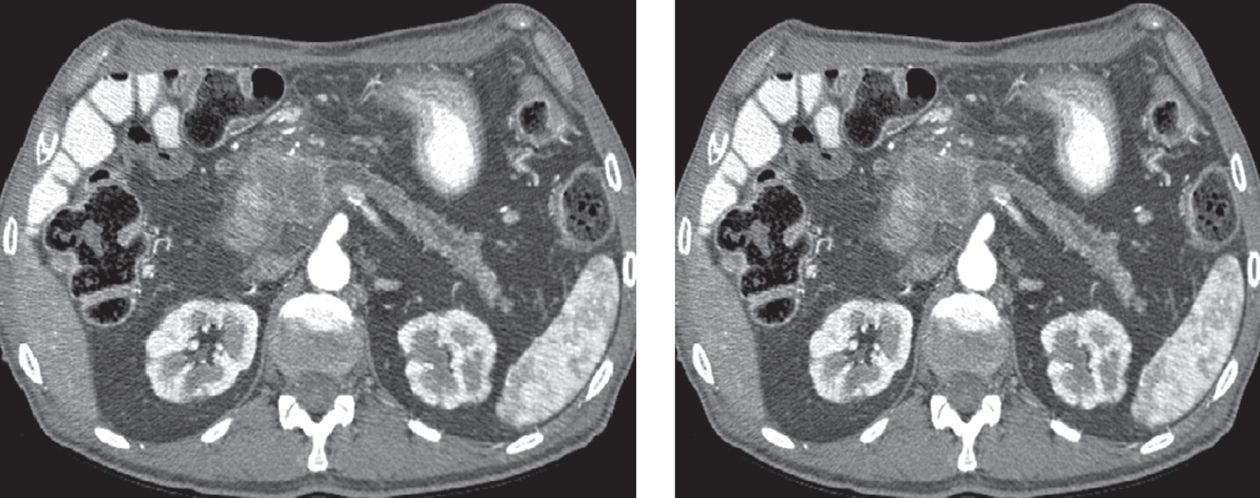
\includegraphics[width=.92\linewidth]{figures/ch06_figure14_data.png}
\par\smallskip
\makebox[.46\linewidth]{原始 CT 图像}\makebox[.46\linewidth]{FPCA 重构图像}
\origfig{14}{晚期胰腺腺癌的原始图像与重构图像。}
\end{figure}

